\subsection{Opportunities with light ions}
\label{sec:jetslightions}

The ability of the LHC to collide ions lighter than Pb as discussed in section \ref{sec:lightions} provides an opportunity to enhance the heavy-ion programme at the LHC with a very large number of rare probes as summarized in section \ref{sec:smallAsum}.  \ArAr\ collisions are used as a test case for light ion running, although the optimal choice of ion is still under study. It is clear that due to the larger integrated luminosity obtainable for a given heavy-ion running period the number of jets produced in \ArAr\ collisions will be significantly larger than in \PbPb\ collisions.  The question which will determine the value of the of light-ion running to the study of jets and parton energy loss is to what extent jet suppression effects will be present in smaller systems.  In this section, projections for \ArAr\ and \XeXe\ collisions at the LHC are considered using the \jewel\ Monte Carlo event generator~\cite{Zapp:2013vla}, to study this question.  

%\subsubsection{Inclusive Jet Energy Loss}
To study the jet nuclear modification factor \RAA\ (discussed in section \ref{sec:preceloss}) in \ArAr\ collisions, within the framework of \jewel\ it is considered as the medium over vacuum ratio of the jet transverse momentum spectrum and
\begin{equation}
    R_{\rm AA}^{\rm jet} = \frac{1/N_{\rm evts}^{\rm med} \rmd N_{\rm jets}/\rmd p_{\rm T}^{\rm med}}{1/N_{\rm evts}^{\rm vac} \rmd N_{\rm jets}/\rmd p_{\rm T}^{\rm vac}} \, ,
\end{equation}
stands in for equation \ref{eq:RAAjet}. Table \ref{tab:medium_pars} summarizes the parameters used in \jewel\ to calculate this quantity in 0--10\% centrality \ArAr\ collisions, compared with the parameterization for \PbPb\ and \XeXe\. The $T_i^{v1}$ values were obtained assuming the same pre-factors as in \cite{Dainese:2016gch}:
\begin{equation}
    T (t) = \left( \epsilon(t) \frac{30}{47.5 \, \pi^2} \right)^{1/4} \, ,
\end{equation}
where the energy density $\epsilon(t)$ follows a Bjorken evolution:
\begin{equation}
    \epsilon(t) = \frac{1}{\pi R_{nucl}^2 t} \frac{dE}{d\eta} \, .
\end{equation}
The energy in central pseudo-rapidity ($dE/d\eta$) is taken from the number of participants and $\sqrt{s_{NN}}$. Finally the temperature $T_i^{v1}$ is evaluated at $\tau_i$.
\begin{table}[!ht]
    \centering
    \begin{tabular}{|c|c|c|c|}
        \hline
         &  \PbPb & \XeXe & \ArAr \\
        \hline
        $\sqrt{s_{NN}}$ (TeV) & 5.02 & 5.80 & 6.30 \\
         $\left\langle N_{\rm part} \right\rangle$ & 353 & 210 & 66\\
         $R_{\rm nucl}$ (fm) & 6.6 & 5.4 & 3.6\\
         $\tau_i$ (fm) & 0.6 & 0.57 & 0.63 \\
         $T_i^{v1}$ (MeV) & 360 & 350 & 318 \\
         $T_i^{v2}$ (MeV) & 260 & 250 & 218 \\
         \hline
    \end{tabular}
    \caption{Energy and medium parameter used in \jewel\ simulation of dijets and Z+jet events.}
    \label{tab:medium_pars}
\end{table}

%Figure \ref{fig:jewel_raa} (left) shows the predicted \RAA\ as a function of the reconstructed jet $p_T$ (in solid lines) together with ATLAS measurements of the same quantity \cite{Aaboud:2018twu} (in filled colored area to account for the experimental uncertainties). The ATLAS centrality classes shown in the figure are chosen to approximately match the $\left\langle N_{part} \right\rangle$ values in Table \ref{tab:medium_pars}. Figure \ref{fig:jewel_raa} (right) shows the \RAA\ for a jet $p_T \in [100-126]$ GeV as a function of the $\left\langle N_{part} \right\rangle$, for ATLAS \PbPb measurements and \jewel calculations for \PbPb, \XeXe, and \ArAr.%. In black are the ATLAS experimental results\cite{Aaboud:2018twu} with the corresponding uncertainties. \jewel\ results for \PbPb\ with $[0-10]\%$ centrality, $[10-20]\%$ centrality and $[40-50]\%$ centrality are shown in red, \XeXe\ $[0-10]\%$ centrality in orange and \ArAr\ $[0-10]\%$ centrality in blue.

%\begin{figure}[!ht]
%\centering
%\includegraphics[width=.45\textwidth,page=3]{figures/jewel/jewel_params_v1.pdf}
%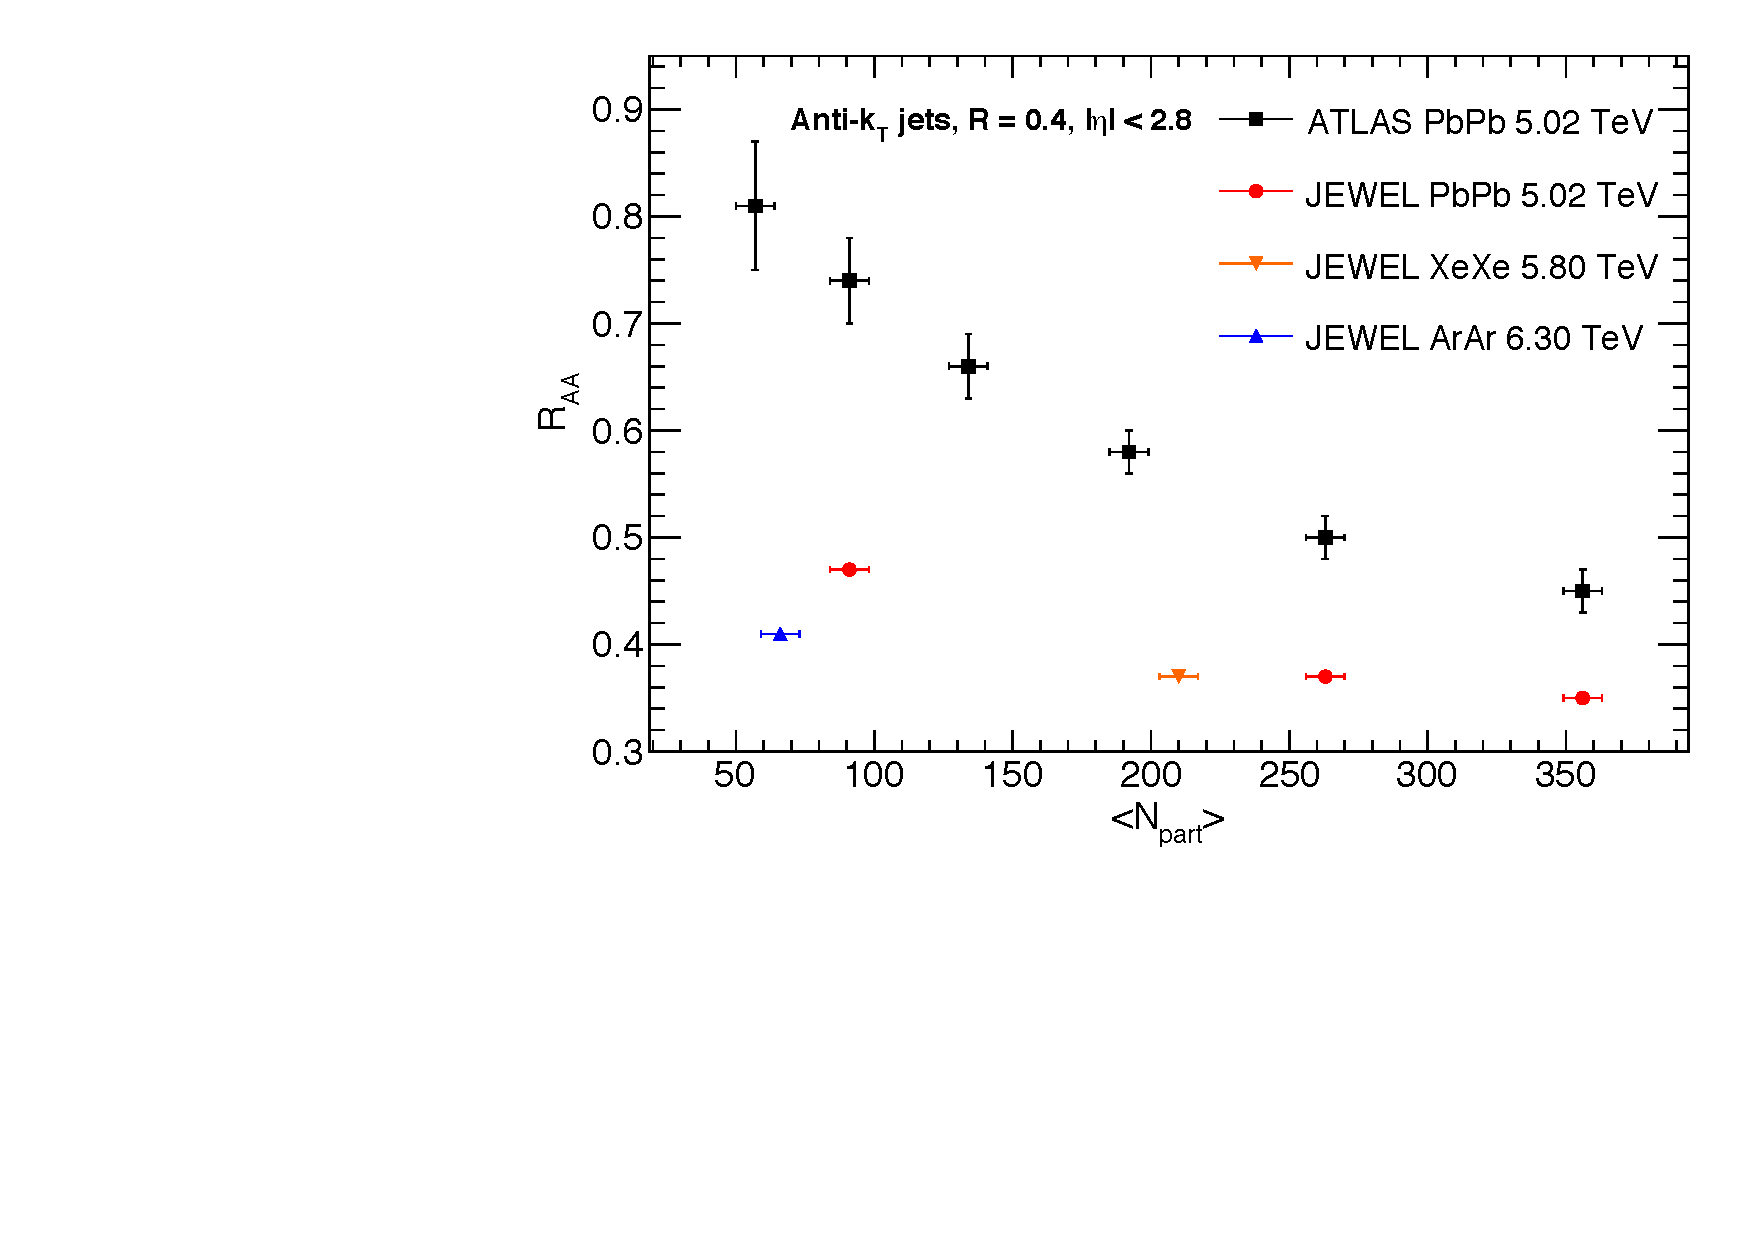
\includegraphics[width=.45\textwidth,page=1]{figures/jewel/jewel_params_v1.pdf}
%\caption{Jet \RAA\ obtained from \jewel\ simulations using the medium parameters listed in Table \ref{tab:medium_pars}, with the temperatures listed as $T_{i}^{v1}$. On the left, the \RAA\ is presented as a function of the jet $p_T$. On the right, \RAA\ as a function of $\left\langle N_{part} \right\rangle$ for a jet $p_T \in [100-126]$~GeV is shown.}
%\label{fig:jewel_raa}
%\end{figure}

With these medium parameters, \jewel\ lies quite below the ATLAS \RAA\ results for the \PbPb\ $[0-10]\%$ centrality class \cite{Aaboud:2018twu}. \jewel was run with medium recoil effects off, although they are known to contribute to increase the jet \RAA\ by $\sim$ 0.1-0.2 in the most central events \cite{KunnawalkamElayavalli:2017hxo} which may explain the discrepancy. Alternatively, the discrepancy can be eliminated by changing the temperature.  With the temperature changed in order to match the ATLAS results for the \PbPb\ $[0-10]\%$ centrality class, temperatures for \XeXe\ and \ArAr\ are obtained by assuming that the energy density scales with $A^{1/3}$. As such, for an arbitrary collision system $XX$:
\begin{equation}
    \left( \frac{T_{XX}}{T_{\rm Pb-Pb}} \right )^{4} = \left( \frac{A_{XX}}{A_{Pb}} \right)^{1/3} \, .
\end{equation}
This parameterisation is used to obtain the $T_i^{v2}$ values listed in Table \ref{tab:medium_pars} which are used to calculate the jet \RAA\ shown in Figure \ref{fig:jewel_raa_v3}.  The figure shows the \jewel calculations for \PbPb, \XeXe, and \ArAr\ along with ATLAS \PbPb\ measurements in centrality classes chosen to match the $\left\langle N_{\rm part} \right\rangle$ values in Table \ref{tab:medium_pars}.

\begin{figure}[!ht]
\centering
\includegraphics[width=.45\textwidth,page=2]{\main/jets/figures/jewel/jewel_params_v3.pdf}
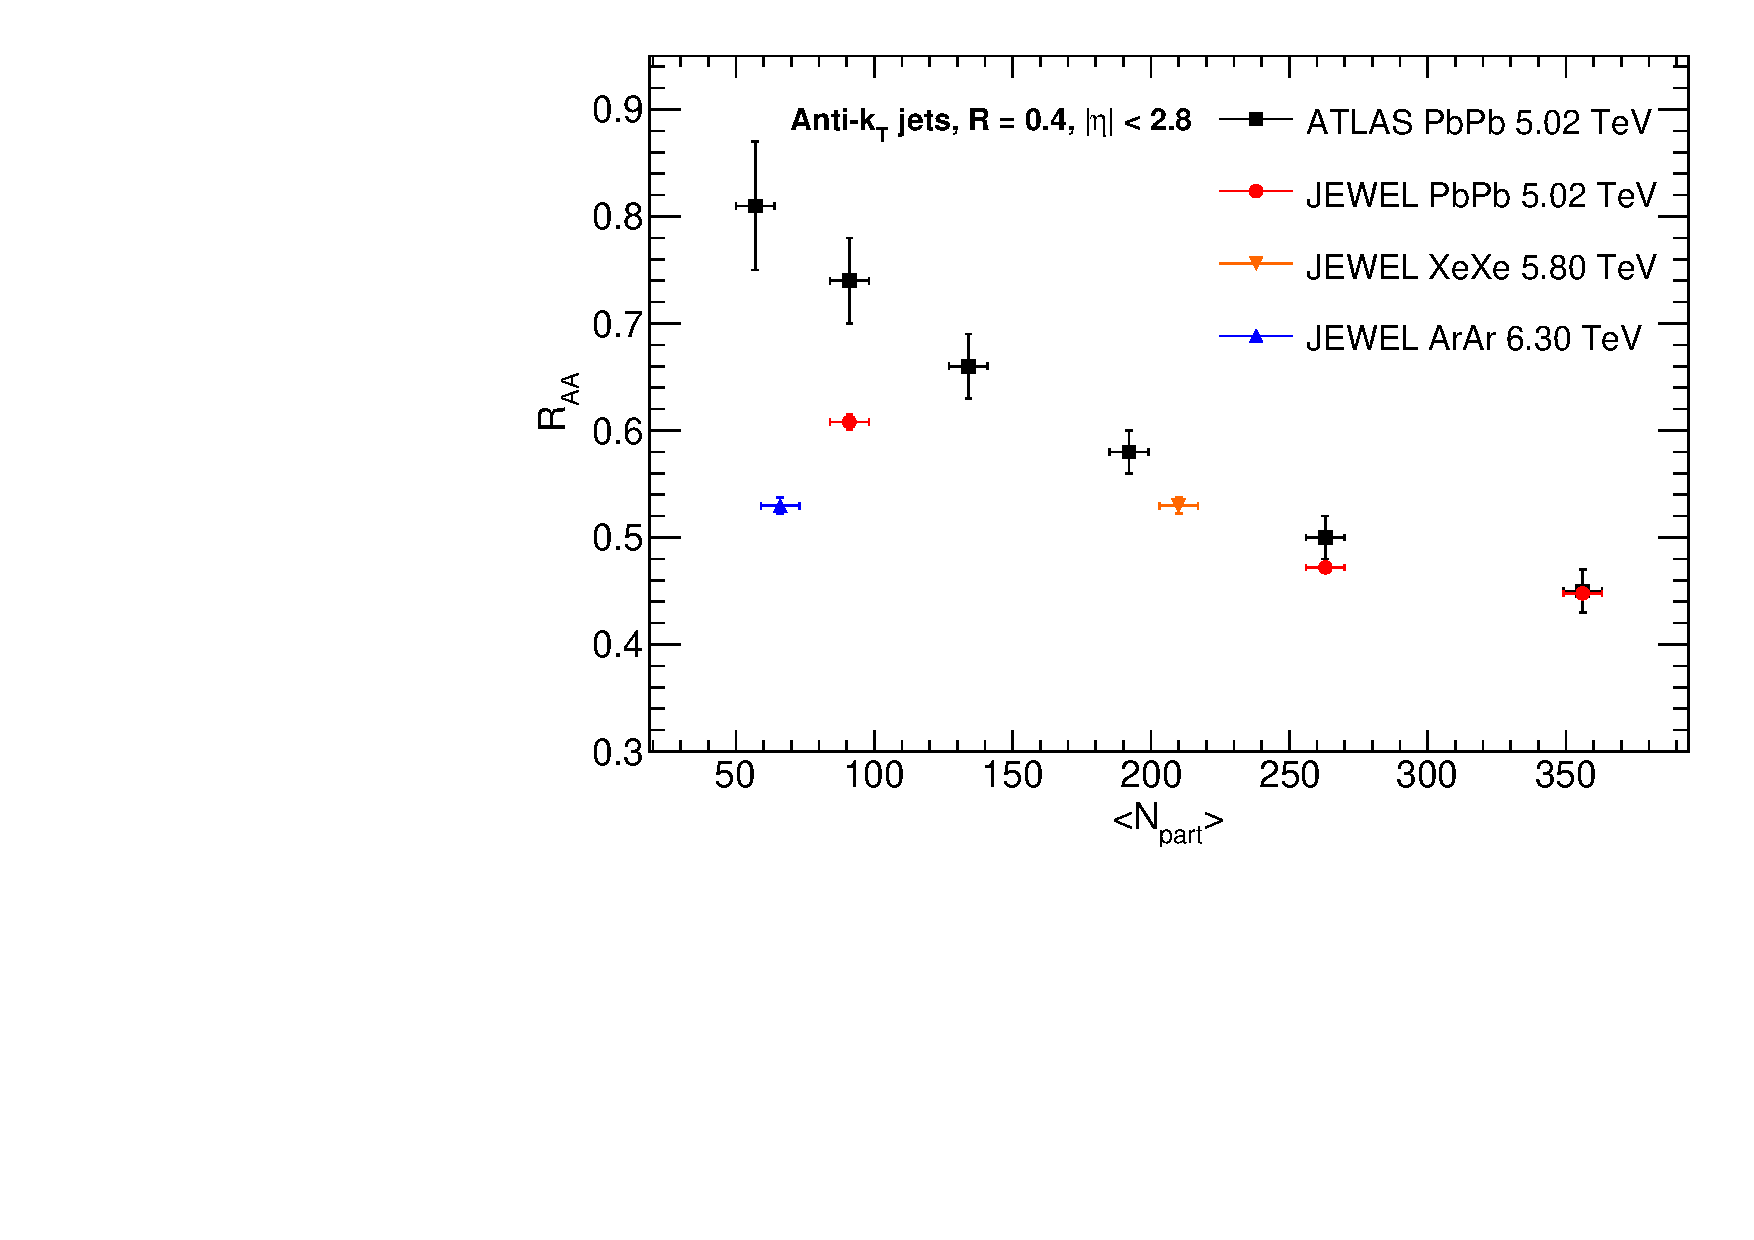
\includegraphics[width=.45\textwidth,page=1]{\main/jets/figures/jewel/jewel_params_v3.pdf}
\caption{Jet \RAA\ obtained from a \jewel\ simulations using the medium parameters listed in Table \ref{tab:medium_pars}, with the temperatures listed as $T_{i}^{v2}$. On the left, the jet \RAA\ is shown as a function of the jet $p_T$, and on the right as a function of $\left\langle N_{\rm part} \right\rangle$ for a jet $p_T \in [100-126]$~GeV.}
\label{fig:jewel_raa_v3}
\end{figure}

%While \PbPb\ central events now follow ATLAS results, there is still an oversuppression for the more peripheral events. A further look into the geometry description within this model would be required to understand the shift with respect to data. Nonetheless, it seems that the results for central collisions are relatively well described within this model. As such, the medium parameters $T_{i)^{v2}$ are taken as reference for the boson + jet events.
To further investigate jet energy loss in \ArAr\ collisions, $Z$ boson + jet events are studied within the same \jewel framework.
%\subsubsection{$Z$ Boson + Jet Energy Loss}
The importance of boson + jet events for the precision study of energy loss is discussed in section \ref{sec:preceloss}.  %To study this in \ArAr collisions,
Events with a $Z$ boson decaying into $\mu^+ \mu^-$ associated with a jet were simulated with \jewel + \pythia Monte Carlo \cite{KunnawalkamElayavalli:2016ttl}. Events were selected for a reconstructed $Z$ boson with a mass within $[70-110]$~GeV, a minimum \pt of 10~GeV for its decay muons, and an associated jet with a $p_T > 30$~GeV and a $|\delta \phi| > 7 \pi/8$ with respect to the boson reconstructed direction. The resulting energy asymmetry distributions, $x_{\mathrm{J}Z}=p_\mathrm{T}^{\textrm{jet}}/p_\mathrm{T}^{Z}$, normalized to the number of reconstructed $Z$ bosons are shown in Figure \ref{fig:jewel_xjz}.% In dashed it is shown the proton-proton reference, in blue the \jewel predictions for \ArAr\ $[0-10]\%$, in filled light red the \PbPb\ $[0-10]\%$ and in green diagonal lines the \PbPb\ $[40-50]\%$ centrality class.

\begin{figure}[!ht]
\centering
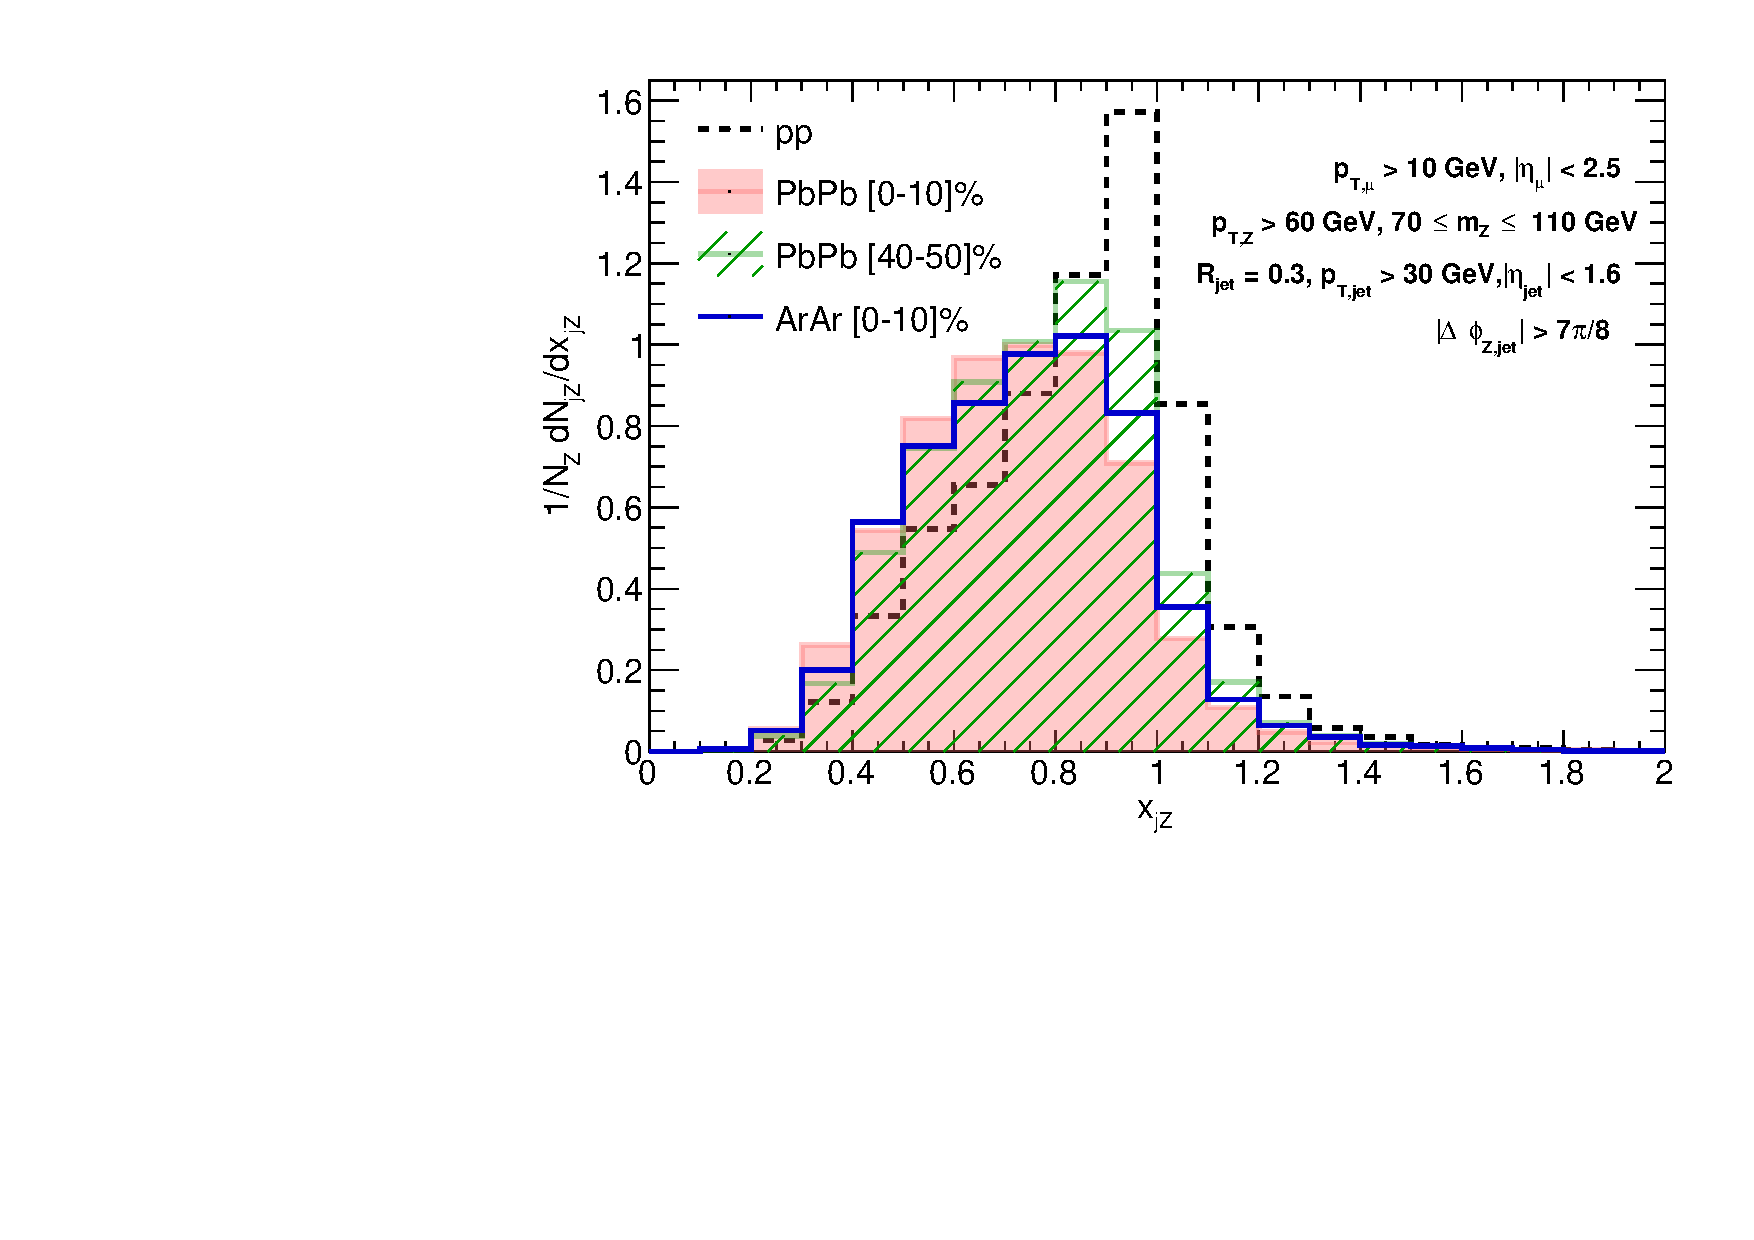
\includegraphics[width=.45\textwidth,page=1]{\main/jets/figures/jewel/jewel_xjz_final.pdf}
\caption{Boson-Jet energy asymmetry, $x_{jZ}$ obtained from \jewel\ simulations using the medium parameters listed in table \ref{tab:medium_pars}, with the temperatures listed as $T_{i}^{v2}$.}
\label{fig:jewel_xjz}
\end{figure}

%This last centrality bin was added in order to have a better estimate on the energy loss of small systems, with the caveat that jet \RAA\ in \jewel\ is below the data for less dense systems. 
Taken together, the above calculations suggest that \jewel does somewhat over-predict suppression in smaller systems, e.g. \XeXe. However, considering that central collisions are reproduced well by this model and that allowing as an upper limit the suppression measured in the \PbPb\ $[40-50]\%$ centrality bin, a significant suppression is expected in central \ArAr collisions.  This is consistent with a simple assumption of $\left\langle N_{\rm part} \right\rangle$ as the controlling parameter in which the value for central \ArAr collisions is within the jet suppression regime \cite{Sirunyan:2018eqi,ATLAS:2018vmo}.  The expected suppression combined with the much larger number of expected jets in \ArAr\ collisions makes lighter ion collisions at the LHC an attractive possibility for the study of jet and parton energy loss.
%To do: Add some information regarding a possible propagation of the 25$\%$ underestimation on ArAr
